\section{Validation}
In this section we will validate and prove that our implementation works as expected and we will look into the performance of the implementation compared to similar alternatives.
\subsection{Benchmark}
When you choose your protocol, performance is an important factor. It should be said that you would probably not want to choose AMQP for its blistering speed, but rather for its broadcast or its queuing abilities or its delivery guarantees. In high performance request-response scenarios peer-to-peer is what you want, but that is not possible with AMQP. Every message is routed through an exchange server. This has a performance strength in the scenario where you broadcast your message once and it is routed to many (thousands) of clients.

For benchmarking we have sought inspiration from the project \textit{Implementation of D-Bus support for Jolie}\cite{D-Bus} as it has an excellent benchmarking suite for Jolie which we have modified for our purpose, but we have modified key parts of it, and have written tests that are relevant for our extension.
\subsubsection{Test hardware}
For the benchmarking we used a quad core machine with 8 logical threads running Ubuntu Desktop 13.10 64-bit. We used RabbitMQ as the AMQP message queue server. RabbitMQ was installed on the same machine but in a virtual PC (VMWare).\\
The performance of AMQP should be slightly better with RabbitMQ running on a real server.\\
The performance in general should be quite a bit worse on a real network instead of a virtual one. Especially for AMQP as AMQP has more network calls.
\begin{itemize}
\item CPU: Intel i7 2.2 GHz quad core with HyperThreading
\item RAM: 8 GB DDR3
\item OS and swap disk: Samsung 840 Evo 1 TB
\item OS: Ubuntu Desktop 13.10 64-bit
\item Jolie version: 1.0
\item Java Runtime Environment version: 1.7.0_45-b18 64bit
\item RabbitMQ OS: Ubuntu Desktop 13.10 64-bit
\item RabbitMQ version: 3.3.1
\item erlang version: R16B01
\item VMWare Player version: 6.0.2
\item vCPUs: 2
\item Virtual RAM: 1 GB
\item Network: VMWare virtual network
\end{itemize}
\subsubsection{RPC calls}
To test RPC calls we have created a server that has one method. This methods gets an integer, and returns twice that. We have then created a client that sends a number requests to that server and exits when the last response has been received. We have measured the time from starting the client to when the client exits. We have used Java to run the Jolie programs through Jolie, to be able to use Java to time the operation. To see the difference from socket and AMQP we have varied the number of requests we sent before closing the client. The number of requests have been between 1,000 and 10,000 with increments of 1,000.

Our results are as follows:

\noindent\begin{tikzpicture}[trim axis left]
  \begin{axis}[
    scale only axis,
    grid=major,
    scaled x ticks=false,
    scaled y ticks=false,
    ylabel=Time in seconds,
    ymin=0,
    ymax=25,
    ytick={0,5,...,25},
    xlabel=Messages,
    xmin=1000,
    xmax=10000,
    xtick=data,
    height=5cm,
    width=\textwidth,
    legend entries={Socket SODEP, AMQP SODEP},
    legend style={at={(0.05,0.95)},anchor=north west},
    axis lines=left
  ]
    \addplot+[smooth]table{onetoone_socket_sodep.data};
    \addplot+[smooth]table{onetoone_amqp_sodep.data};
  \end{axis}
\end{tikzpicture}

It is quite obvious here that AMQP is not suited for RPC-style calls as we have mentioned earlier. AMQP is between 50 \% and 75 \% slower than socket at RPC calls at the tested interval.

\subsubsection{One publisher, multiple subscribers}
To test a likely scenario where the architect would choose AMQP, we designed a test where we have a publisher that sends 1,000 messages to a number of subscribers. Having the AMQP server enables us to send the messages no more than once as AMQP handles routing to the subscribers, but for socket we have to duplicate the messages so that each subscriber gets one. We measure the time it takes for the publisher to publish all its 1,000 messages. We do not wait for subscribers to handle them. The method defined in the interface is a one-way method for SODEP and SVDEP, but SOAP failed when there was no response, so for SOAP we had to create a method that returns an empty response. To really see the difference we varied the number of subscribers from 1 to 10.

Our results for using SOAP as the protocol is:

\noindent\begin{tikzpicture}[trim axis left]
  \begin{axis}[
    scale only axis,
    grid=major,
    scaled x ticks=false,
    scaled y ticks=false,
    ylabel=Time in seconds,
    ymin=0,
    ymax=300,
    ytick={0,50,...,300},
    xlabel=Subscribers,
    xmin=1,
    xmax=10,
    xtick=data,
    height=5cm,
    width=\textwidth,
    legend entries={Socket SOAP, AMQP SOAP},
    legend style={at={(0.05,0.95)},anchor=north west},
    axis lines=left
  ]
    \addplot+[smooth]table{onetomany_socket_soap.data};
    \addplot+[smooth]table{onetomany_amqp_soap.data};
  \end{axis}
\end{tikzpicture}


And our results for using SODEP/SVDEP is:

\noindent\begin{tikzpicture}[trim axis left]
  \begin{axis}[
    scale only axis,
    grid=major,
    scaled x ticks=false,
    scaled y ticks=false,
    ylabel=Time in seconds,
    ymin=0,
    ymax=25,
    ytick={0,5,...,25},
    xlabel=Subscribers,
    xmin=1,
    xmax=10,
    xtick=data,
    height=5cm,
    width=\textwidth,
    legend entries={Socket SODEP, AMQP SODEP, AMQP SVDEP},
    legend style={at={(0.05,0.95)},anchor=north west},
    axis lines=left
  ]
    \addplot+[smooth]table{onetomany_socket_sodep.data};
    \addplot+[smooth]table{onetomany_amqp_sodep.data};
    \addplot+[smooth]table{onetomany_amqp_svdep.data};
  \end{axis}
\end{tikzpicture}


As both graphs show AMQPs execution-time is not dependent on the number of subscribers, and this is one of AMQPs strengths. Another one of AMQP's strengths are that we do not have to wait for confirmation like we do for socket. We still have guarantee for delivery. We can see that AMQP is faster already when we have two subscribers.
\subsubsection{Conclusion}
AMQP performs better than we expected. AMQP is always out performed by socket for peer-to-peer transmissions which was not surprising, but we found AMQP surprisingly fast considering how direct socket is and how little overhead it has.

As expected AMQP had an huge advantage for broadcasting a message to many subscribers. AMQP out performs socket as soon as you have just two recipients no matter the size of the message. The difference was the least between socket and AMQP when using SODEP because of the limited overhead for each message.
\subsection{The JoRBA Project}
\label{subsec:The JoRBA Project}
The JoRBA Project\cite{Jorba} (Jolie Rule-Based Adaptation framework) is a project about dynamic adaptation through the use of hooks and adaptation rules.

The project includes proof of concept software which is fairly large distributed system of communicating components. We downloaded the software and modified nothing but the location fields so it used our AMQP extension and our RabbitMQ message queue server as a relay for the communication between the components. We started seven components and they registered with the adaptation manager and the test client ran perfectly.

This was a great test of our request-response implementation.
\begin{figure}[H]
  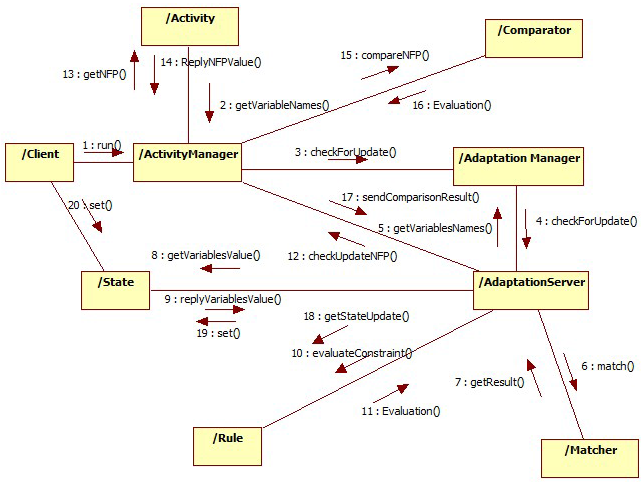
\includegraphics[width=\textwidth]{illustrations/Jorba.png}
  \caption{JoRBA collaboration diagram}
\end{figure}
\newpage
